\subsection{Can Lighting Requirements Be Met Through the Proposed System?}

\paragraph{}
For lighting requirements, as previously discussion in Section \ref{section:draft-floor-plan} there are Australian standards that impact the quantity and types of luminaires. Table \ref{table:LightingRequirements} outlines the lux requirements expressed in AS/NZS 1680.2.2 explaining that the target for a standard office should be between 200\,lux and 300\,lux unless technical work is required (a minimum of 320 is required in this case) \cite{StandardsAustralia2006_2}.

\paragraph{}
To begin the analysis, the project test model standard office was modelled in the lighting simulation software package Dialux. As discussed in Section \ref{section:project-model} the floor plan is based off of QUT Garden's Point Campus P Block level 6. The reason this was chosen is that it is a real world application of a commercial office floor that access to the schematics and design plans was made available. This was the most accurate method for producing a model that could be applied to industry. 

\subsubsection{Office Room Lighting Model}   

\paragraph{}
The large floor plan shown in Section \ref{section:draft-floor-plan} was loaded into Dialux and an office separated out for modelling. The room was approximation shows that offices on this are 22\,\si{m^2} and this lighting simulation displays this. The fittings modelled were luminaires with the same specifications outlined in the QUT design documents. Specifically, this is the Futcha LED 27.5W fitting from Pierlite \cite{website:Pierlite1}. The DWG file additionally outlined some architectural objects including a table which was included in the modelling. 

\paragraph{}
When modelling in Dialux, assumptions are required for things like roof heights, luminaire mounting heights and surface reflectances. Following building standards Table \ref{table:QUT-lvl6-office-assumptions} below outlines the assumptions made in the completed lighting analysis. 

\begin{table}[htb]
	\centering
	\renewcommand{\arraystretch}{2}
	\begin{tabular}{|l|l|}
		\hline
		\textbf{Assumption} & \textbf{Value} \\ \hline
		Roof Height         & 2.7m           \\ \hline
		Workplane           & 0.75m          \\ \hline
		Boundaries          & 0.1m           \\ \hline
		Ceiling Reflectance & 70\%           \\ \hline
		Wall Reflectance    & 50\%           \\ \hline
		Floor Reflectance   & 20\%           \\ \hline
	\end{tabular}
	\caption{QUT: P Block Level 6 Office Lighting Simulation Assumptions}
	\label{table:QUT-lvl6-office-assumptions}
\end{table}  

\paragraph{}
This calculation was completed as a test basis to ensure that the information received from the schematics were correctly understood. Appendix \ref{appendix:QUT-Lvl6-office-rev3} shows the complete report however the important aspects are of course the lux values throughout the workplace shown in Figure \ref{fig:dialux-office-workplane-summary} and the 3D render for visual appeal shown in Figure \ref{fig:dialux-office-3D}.  

\begin{figure}[H]
	\hfill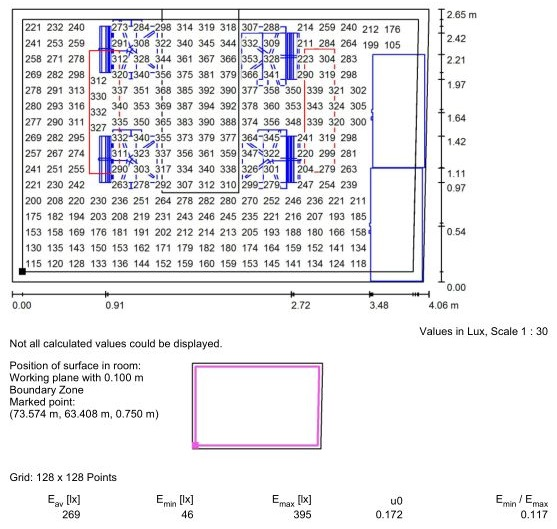
\includegraphics[width = 150mm]{images/project-model/dialux-office-workplane-summary}\hspace*{\fill}
	\caption{QUT: P Block Level 6 Office Lux Analysis} 
	\label{fig:dialux-office-workplane-summary}
\end{figure}

\begin{figure}[H]
	\hfill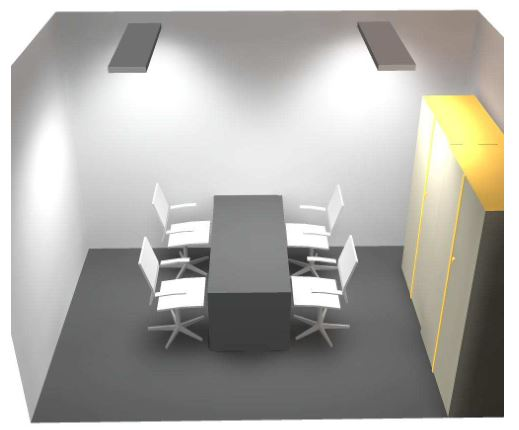
\includegraphics[width = 150mm]{images/project-model/dialux-office-3D}\hspace*{\fill}
	\caption{QUT: P Block Level 6 Office 3D Render} 
	\label{fig:dialux-office-3D}
\end{figure}

\subsubsection{Lighting Model Discussion}

\paragraph{}

\newline
***TO BE COMPLETED***


\subsubsection{DC Light Devices}

\paragraph{}
***TO BE COMPLETED***

